\documentclass[12pt]{aghdpl}
\usepackage{hyperref}

\author{Mateusz Woźniak}
\shortauthor{M. Woźniak}

\titlePL{Klasyfikacja wybranych komórek szpiku kostnego na podstawie zdjęć rozmazów przy użyciu algorytmu opartego na splotowych sieciach neuronowych}
\titleEN{Classification of selected bone marrow cells from smear images using convolutional neural networks}


% Dopuszczalne wartości[1,2]:
% * "Projekt dyplomowy" - na koniec studiów I stopnia
% * "Praca dyplomowa" - na koniec studiów II stopnia
% [1] Zasady dyplomowania w roku akademickim 2020/2021 (Decyzja Dziekana WEAIiIB nr 16/2020 z dnia 9 grudnia 2020 roku)
% [2] Załącznik nr 1a) do Decyzji nr 16/2020 Dziekana Wydziału EAIiIB z dnia 09 grudnia 2020 r.
\thesistype{Projekt dyplomowy}

\supervisor{dr Tomasz Hachaj}

\degreeprogramme{Informatyka i Systemy Inteligentne}

\date{2024}

%\department{Katedra Informatyki Stosowanej}
%\department{Department of Applied Computer Science}

\faculty{Wydział Elektrotechniki, Automatyki, Informatyki i Inżynierii Biomedycznej}

\acknowledgements{\small{Niniejszą pracę chciałbym zadedykować moim wspaniałym
\mbox{Rodzicom \textbf{Joannie i Wojciechowi Woźniak},} którzy wspierali
mnie w całym okresie studiów,
    pokazali wartość nauki oraz wykszałcili szacunek do niej.
    \newline
    \newline
    Za wiedzę i wsparcie w poznaniu zagadnień medycznych,
    pragnę wyrazić serdeczne podziękowania dla \textbf{lek. Macieja Błądzińskiego}.
    Jego zaangażowanie było niezwykle pomocne w zrozumieniu wyzwań, z jakimi mierzy się nowoczesna medycyna.
    \newline
    \newline
    Za wyrozumiałość, inspirację oraz pomoc pragnę złożyć serdecznie podziękowania mojemu
    promotorowi \textbf{dr hab. inż. Tomaszowi Hachajowi}. Jego oddanie, profesjonalizm i~cenne rady stanowiły nieocenioną wartość w trakcie realizacji tego projektu.
}}


\begin{document}

    \titlepages
    \RedefinePlainStyle

    \setcounter{tocdepth}{2}
    \tableofcontents
    \clearpage

%	\include{rozdzial1}
%	\include{rozdzial2}
%	\include{rozdzial3}
%	\include{tests}

    \chapter{Wstęp}


\section{Wprowadzenie}

Rozwój technologii informatycznych, w szczególności uczenia maszynowego, otwiera nowe możliwości w wielu dziedzinach nauki i przemysłu.
Jednym z obszarów życia, w którym te technologie mogą odnieść duży sukces, jest medycyna.
Zastosowanie komputerów do analizy danych medycznych powoduje polepszenie procesów leczenia wielu chorób.
Sztuczna inteligencja daje możliwość zautomatyzowania czasochłonnych zadań w diagnostyce i zaoszczędzenie wielu godzin pracy lekarza diagnosty.

Celem niniejszej pracy jest zastosowanie splotowych sieci neuronowych do klasyfikacji komórek szpiku kostnego na podstawie zdjęć rozmazów.
Wykorzystanie tej technologii może znacznie przyspieszyć i ułatwić proces diagnozy, co jest kluczowe dla skutecznego leczenia wielu chorób takich jak nowotwory krwi.

Praca ma charakter badawczy i jest próbą zastosowania nowoczesnych technologii informatycznych w praktycznym problemie medycznym.


\section{Motywacja}

W ostatnich latach obserwuje się coraz większe zastosowanie informatyki, a w szczególności algorytmów uczenia maszynowego,
w medycynie i diagnostyce.
Jednym z ważniejszych zastosowań jest wykorzystanie widzenia komputerowego, wspieranego sieciami neuronowymi, do przetwarzania i analizy obrazów medycznych.
Przykładowo odpowiedni system może analizować wyniki tomografii komputerowej bądź rezonansu magnetycznego, by stwierdzać niepokojące zmiany w ciele człowieka.
Odpowiednia sieć neuronowa widzenia komputerowego może na przykład badać skany ludzkiego mózgu i ustalać, czy na zdjęciu jest widoczny guz \cite{brain_tumor}.
Innym przykładem jest traktowanie zapisu sygnału elektrokardiogramu jako szerokiego
obrazu \cite{ecg_cnn}.
Wtedy program komputerowy może oznaczać fragmenty, na które lekarz powinien zwrócić szczególną uwagę.

W niniejszym projekcie zaproponowany algorytm uczenia maszynowego jest w stanie rozpoznawać komórki w szpiku kostnym.
Klasyfikowanie typów komórek jest kluczowe z perspektywy diagnostyki wielu chorób.
Przykładowo stwierdzenie ostrej białaczki limfoblastycznej opiera się na m.in.
zliczeniu 1000 komórek i policzeniu, ile z nich jest limfoblastami~\cite{blast_counting_diagnosis}.
Obecnie nie istnieje w pełni automatyczny system ich zliczania, więc w procesie diagnostyki musi być zaangażowany człowiek.
Postęp w tym zakresie oznaczałby znaczne przyspieszenie diagnozy pacjenta, a co za tym idzie polepszenie rokowania wyleczenia.


\section{Cele i zakres pracy}

Celem pracy jest porównanie kilku algorytmów uczenia maszynowego z wykorzystaniem splotowych sieci neuronowych do rozpoznawania typów komórek na podstawie zdjęć.
Zdjęcia przedstawiają obraz mikroskopowy rozmazu szpiku kostnego. Wykorzystany zbiór danych pochodzi z
Monachijskiego Labolatorium Białaczek (\textit{MLL Münchner Leukämielabor} \cite{mll}) i jest dostępny na platformie \textit{kaggle.com} \cite{dataset}.
Praca ma za zadanie porównać różne architektury splotowych sieci neuronowych i stwierdzić, która z nich daje najlepsze rezultaty.

Praca zawiera także omówienie algorytmu wstępnego przetwarzania danych (z ang. \textit{preprocessing}) oraz algorytmu ekstrakcji obrazów komórek z dużego skanu rozmazu.

    \chapter{Zagadnienia teoretyczne}


\section{Sieci neuronowe}

Sieci neuronowe stanowią jedną z najpopularniejszych technik uczenia maszynowego. Są one inspirowane działaniem ludzkiego mózgu. Sieci składają się z neuronowów, pogrupowanych w połączone ze sobą warstwy.

Ogólna architektura sieci neuronowej:
\begin{itemize}
    \item Warstwa wejściowa - ta warstwa przyjmuje dane początkowe w formie tensora liczb rzeczywistych. Danymi wejściowymi mogą być poziomy jasności obrazu, dane o cenach lub sygnale (w przypadku prognozowania serii czasowych) lub osadzenia (z ang \textit{embeddings}) dla modeli językowych.
    \item Warstwy ukryte - te warstwy przetwarzają dane wejściowe przez sekwencję transformacji matematyczncyh. Neurony są połączone z poprzednią warstwą, a siła ich połączenia jest wyrażana przez tak zwane wagi. Wartość, którą przyjmie dany neuron jest liczona na podstawie ważonej sumy wartości neuronów z poprzedniej warstw. Po obliczeniu sumy, stosowana jest funkcja aktywacji. Ma ona za zadanie wprowadzić nieliniowość obliczeń, która jest wymagana do rozpoznawania zaawansowanych wzorców.
    \item Warstwa wyjściowa - warstwa, która generuje końcowy tensor. Tensor może zawierać informacje takie jak rozkład prawdopodobieństwa przyporządkowania do poszczególnych klas. Może również zawierać prognozowaną liczbę, w przypadku modeli regresyjnych.
\end{itemize}

Proces trenowania sieci neuronowej polega na modyfikowaniu wag pomiędzy połączeniami poszczególnych neuronów tak, by minimalizować różnicę między tensorem wyjściowym, a tensorem oczekiwanym.
Najczęściej stosuje się do tego zadania algorytmy optymalizacyjne oparte na pochodnych i gradientach. Przykładem może być \textit{algorytm spadku wzdłuż gradientu}.
W rzeczywistych zadaniach stosuje się jednak bardziej wyszukane algorytmy takie jak \textit{algorytm stochastycznego spadku wzdłuż gradientu} albo \textit{algorytm Adam}.

Sieci neuronowe okazały się dużym sukcesem w wielu trudnych zadaniach uczenia maszynowego.
Są z powodzeniem stosowane w takich branżach jak medycyna, rozrywka, cyberbezpieczeństwo czy motoryzacja. Na przykład zespół Tesla Vision trenuje duże sieci neuronowe by stworzyć pojazd autonomiczny, zdolny poruszać się bezpiecznie bez kierowcy.
Sieci neuronowe coraz częściej będą wykonywać określone zadania szybciej i skuteczniej niż człowiek.
Czas reakcji systemu autopilot samochodu autonomicznego jest znacznie krótszy niż czas reakcji kierowcy, co w długiej perspektywie może przyczynić się do zwiększenia bezpieczeństwa na drogach i szlakach komunikacyjnych.
Innym bardzo ważnym zastosowaniem sieci neuronowych jest medycyna. Naukowcy z Google DeepMind stworzyli model \textit{AlphaFold}, który jest w stanie przewidywać molekularną strukturę białek.
Postęp informatyki w naukach biologicznych i chemicznych otwiera perspektywę na leczenie chorób, które dotychczas były nieuleczalne i umożliwia lepsze zrozumienie organizmu człowieka.

\section{Propagacja wsteczna}

%TODO backprop

\section{Splotowe sieci neuronowe}

Splotowe sieci neuronowe to rodzaj sieci neuronowych dedykowany do rozpoznawania przede wszystkim cech obrazów.
Znajdują one zastosowanie w zadaniach takich jak klasyfikacja obrazów, rozpoznawanie obiektów lub segmentacja.
Czasem są one używane do analizy wideo lub analizy sygnału w czasie.

Struktura splotowych sieci neuronowych sprowadza się do:
\begin{itemize}
    \item Warstwa wejściowa - ta warstwa przyjmuje zazwyczaj obraz jako tensor jasności poszczególnych pikseli.
    Obraz wejściowy może być w skali szarości (pojedynczy kanał) lub kolorowy - najczęściej składowe RGB pojedynczego piksela są kodowane przez 3 neurony.
    \item Warstwy splotowe - te warstwy wykorzystują matematyczną operację splotu.
    Taka warstwa zawiera pewną macierz, zwaną filtrem o pewnym ustalonym rozmiarze (najczęściej \textit{3x3} lub \textit{5x5}).
    Macierz ta jes przesuwana od lewej do prawej, z góry do dołu po obrazie.
    Odpowiednie wartości filtra są w stanie wzmocnić lub osłabić pewne cechy obrazu takie jak ostre krawędzie bądź rogi.
    Wartości macierzy są dobierane w procesie trenowania modelu.
    \item Warstwy łączące - warstwy te mają za zadanie zmniejszyć wymiarowość danych z poprzedniej warstwy.
    Popularną funkcją łączącą jest uśrednianie - dla zadanego otoczenia pikseli (najczęściej \textit{2x2} lub \textit{3x3}) wybierana jest średnia wartość.
    Inną funkcją łączącą jest maksimum - z otoczenia wybierana jest wartość maksymalna.
    \item Warstwy gęste - po kilku warstwach splotowych, zaawansowane rozumowanie jest przeprowadzane przez warstwy gęste, czyli neurony połączone w sposób "każdy z każdym".
\end{itemize}

Główne zastosowanie splotowych sieci neuronowych:
\begin{itemize}
    \item wykrywanie przedmiotów i ludzi na obrazach i nagraniach wideo
    \item analiza i wykrywanie anomalii w skanach medycznych
    \item pojazdy autonomiczne - analiza sytuacji na drodze
\end{itemize}

W niniejszej


\section{Architektury sieci neuronowych}



\section{Problem klasyfikacji komórek krwi w rozmazach szpiku kostnego}


\section{Konwencjonalne algorytmy widzenia komputerowego}


\section{GradCAM - wytłumaczalne uczenie maszynowe}
    \chapter{Realizacja projektu}


\section{Wykorzystane technologie}

\subsection{Język programowania Python}

Kod projektu został napisany w języku Python. Wybór tego języka był spowodowany szeroką dostępnością bibliotek i
narzędzi wspomagających uczenie maszynowe. W szczególności należy zwrócić uwagę na biblioteki \textit{PyTorch} (użyta w projekcie) oraz \textit{Tensorflow} (alternatywa).
Są to dwie najpopularniejsze biblioteki do operowania na tensorach (tensor to uogólnienie macierzy na wiele wymiarów).
Obie pozwalają na przyśpieszanie obliczeń z użyciem zewnętrznych akceleratorów takich jak np. karty graficzne.

Podczas prac badawczych, wykorzystana wersja Pythona to \textit{3.12.0}.

\subsection{Biblioteka PyTorch}

Biblioteka PyTorch jest obecnie najpopularniejszą biblioteką uczenia maszynowego.
Pozwala ona projektować obliczenia w formie modułów i posiada silnik automatycznego różniczkowania grafu obliczeniowego (z ang. \textit{autograd}).
Owy silnik jest kluczowy z perspektywy trenowania sieci neuronowych, ponieważ jest w stanie optymalizować parametry modelu.
Warto zwrócić uwagę na to, że PyTorch stawia nacisk na przejrzystość obliczeń - dla porównania operacje w Tensorflow są nierzadko
ukryte pod gotowymi funkcjami (zob. listing~\ref{lst:tensorflow_sample} i~\ref{lst:pytorch_sample})

\begin{lstlisting}[language=ipython,caption={Przykładowa sieć neuronowa w Tensorflow},label={lst:tensorflow_sample}]
tensorflow_model = tf.keras.Sequential([
    tf.keras.layers.Flatten(input_shape=(28, 28)),
    tf.keras.layers.Dense(128, activation='relu'),
    tf.keras.layers.Dense(10, activation='softmax')
])

tensorflow_model.compile() # Brak doglebnej kontroli nad przeplywem obliczen
\end{lstlisting}


\begin{lstlisting}[language=ipython,caption={Przykładowa sieć neuronowa w PyTorch},label={lst:pytorch_sample}]
class PyTorchNetwork(nn.Module):
    def __init__(self):
        super(Net, self).__init__()
        self.flatten = nn.Flatten()
        self.fc1 = nn.Linear(28 * 28, 128)
        self.relu = nn.ReLU()
        self.fc2 = nn.Linear(128, 10)

    def forward(self, x): # Dokladna kontrola nad przeplywem obliczen
        x = self.flatten(x)
        x = self.fc1(x)
        x = self.relu(x)
        x = self.fc2(x)
        return x
\end{lstlisting}

PyTorch oferuje również zestaw narzędzi do przetwarzania danych, dostarcza również gotowe, pretrenowane modele dla najpopularniejszych architektur.
Przykładami są pakiety \textit{torchvision} lub \textit{torch.utils}. Biblioteka jest w stanie wykorzystywać karty graficzne (z ang. \textit{graphical processing unit, GPU}) do przyspieszania obliczeń.

\subsection{Biblioteka OpenCV}

Biblioteka OpenCV \cite{opencv} dostarcza implementacje wielu algorytmów wizji komputerowej.
OpenCV \textcolor{red}{zawiera} interfejs programistyczny, dzięki któremu programista Pythona może komunikować się z implementacją algorytmów w C++.
To zapewnia szybkość wykonywania obliczeń, jednocześnie nie wymuszając na programiście pisania kodu w C++. Przykład wykorzystania biblioteki OpenCV widoczny jest na listingu \ref{lst:opencv_sample}
- kod wylicza momenty Hu.

OpenCV w niniejszym projekcie jest wykorzystywane do automatycznej ekstrakcji obrazów z komórkami na podstawie dużego zdjęcia spod mikroskopu.
Więcej informacji na ten temat znajduje się w rozdziale \ref{sec:kwadraty}.

\begin{lstlisting}[language=ipython,caption={Obliczenie momentów Hu z użyciem OpenCV}, label={lst:opencv_sample}]
import cv2

image = cv2.imread('obraz.jpg', 0)  # 0 oznacza wczytanie obrazu w odcieniach szarosci

hu_moments = cv2.HuMoments(cv2.moments(image)).flatten()

print("Momenty Hu:")
for i in range(0, 7):
    print(f"Moment {i+1}: {hu_moments[i]}")
\end{lstlisting}

\subsection{Inne narzędzia}

Kod źródłowy projektu jest przechowywany w repozytorium na platformie GitHub (dostępny pod adresem \url{https://github.com/matisiekpl/thesis}).
Wykresy były generowane za pomocą biblioteki \textit{matplotlib} \cite{matplotlib},
a metryki liczone z użyciem funkcji pakietu \textit{scikit-learn} \cite{scikit_learn}.

\subsection{Sprzęt}

Do prac badawczych został użyty Apple Macbook Pro 2020 (M1/16GB pamięci).
Trenowanie sieci odbywało się na platformie \textit{kaggle.com}, która oferuje bezpłatne 30 godzin obliczeń co miesiąc z kartą graficzną \textit{NVIDIA P100}.


\section{Zbiór danych}

Wykorzystany w projekcie zbiór danych to kolekcja 170 tysięcy zdjęć komórek z rozmazów szpiku kostnego.
Zdjęcia mają nadane etykiety przez diagnostów i przedstawiają różne komórki widziane pod mikroskopem.
Próbki szpiku kostnego pochodzą z biopsji 945 pacjentów z Monachijskiego Labolatorium Białaczek (\textit{MLL Münchner Leukämielabor} \cite{mll}).
Akwizycja obrazu polegała na wykonaniu zdjęcia mikroskopią Brightfield'a~\cite{microscopy} z 40-krotnym powiększeniem.
Producentem mikroskopu było przedsiębiorstwo Fraunhofer IIS.

\begin{figure}
    \includegraphics[width=\textwidth]{images_count}
    \caption{Histogram rozkładu próbek w klasach w zbiorze danych}
    \label{fig:images_count_vis}
\end{figure}

\begin{figure}
    \centering
    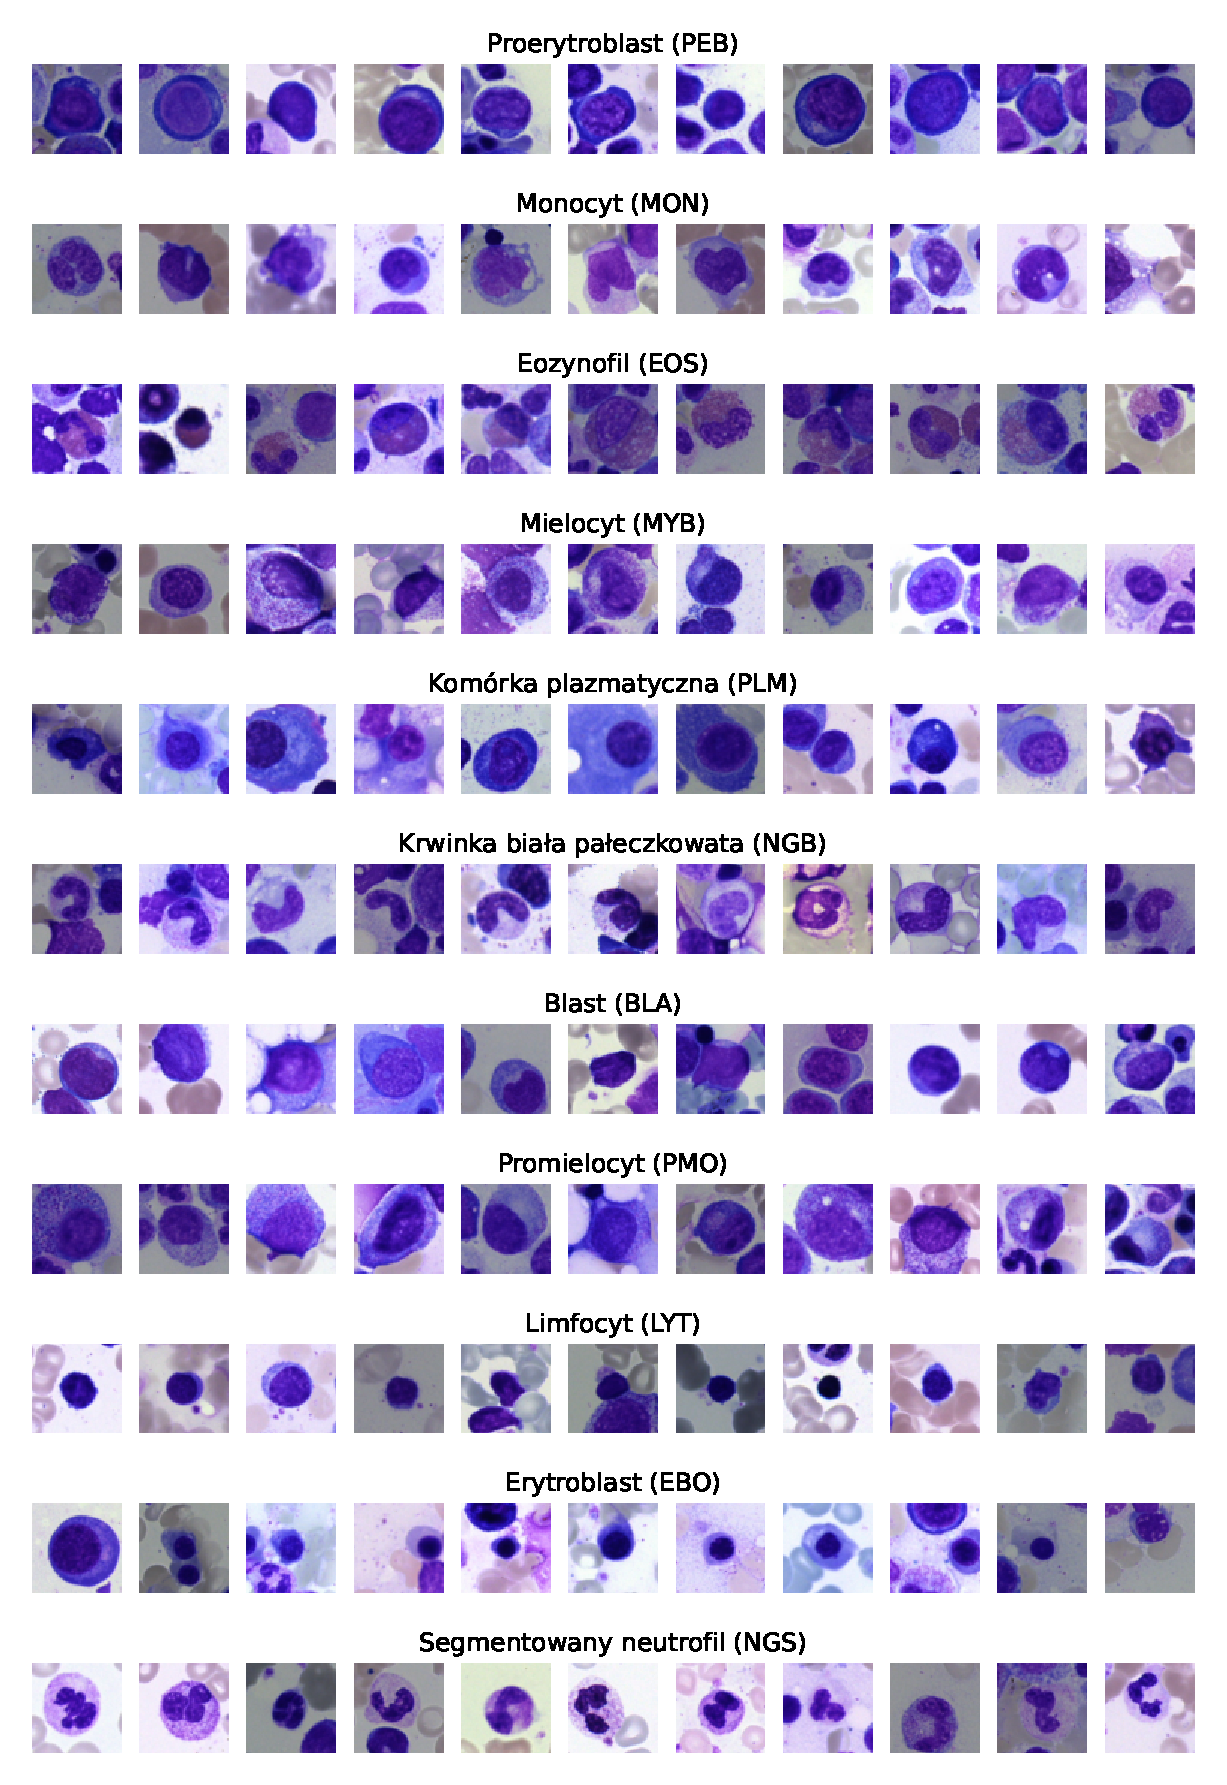
\includegraphics[height=0.9\textheight]{images_examples}
    \caption{Przykładowe zdjęcia komórek ze zbioru danych dla każdej z klas}
    \label{fig:images_examples}
\end{figure}

Komórki były barwione metodą Maya-Grünwalda-Giemsa \cite{histology}.
Zbiór danych zawiera 21 klas, lecz w trakcie trenowania sieci neuronowych wykorzystano jedynie 11 (odrzucone klasy posiadały bardzo małą ilość próbek).
Histogram rozkładu klas jest widoczny na rys. \ref{fig:images_count_vis}.
Zbiór danych jest niezrównoważony, ponieważ ilość obrazów w każdej klasie znacząco się różni.
Przykładowe zdjęcia są widoczne na rys \ref{fig:images_examples}.


\section{Struktura projektu}

\subsection{Przygotowanie danych}

Zbiór danych to katalog ze zdjęciami.
Zdjęcia są pogrupowane w podkatalogach, gdzie jego nazwa oznacza typ komórki.
Każdy podkatalog zawiera kolorowe zdjęcia w formacie \textit{.jpg} w rozmiarze \textit{250 pikseli x 250 pikseli}.
Przed treningiem sieci neuronowej konieczne jest przetwarzanie wstępne zbioru danych (z ang. \textit{preprocessing}).

\begin{lstlisting}[language=ipython,caption={Transformacja danych}, label={lst:transforms}]
transform = transforms.Compose([
    transforms.Resize((224, 224)), # przeskaluj obrazy
    transforms.RandomEqualize(1), # wyrownaj histogram z prawdopodobienstwem 1, czyli dla kazdego obrazu
    transforms.ToTensor(), # zamien na Tensor
    transforms.Normalize(mean=[0.485, 0.456, 0.406], std=[
        0.229, 0.224, 0.225]), # normalizuj wedlug mediany i odch. stand.
])
\end{lstlisting}

Do realizacji przygotowania danych wykorzystano pakiet \textit{torchvision.transforms}.
Kod transformacji jest przedstawiony na listingu~\ref{lst:transforms}.
Wykonuje on przeskalowanie obrazu wejściowego do rozmiaru \textit{224 piksele na 224 piksele}.
Następnie wyrównuje histogram i normalizuje według średniej i odchylenia standardowego (rys.~\ref{fig:transformations_example}).

Wyrównanie histogramu jest konieczne z powodu różnic w odcieniach barwienia Maya-Grünwalda-Giemsa~\cite{stain}.
Przy każdym wykonaniu rozmazu intensywność kolorów komórek jest inna.
Taka normalizacja zapobiega błędnemu nauczeniu się sieci neuronowej ze względu na odcień, a nie kształt i wygląd komórek.

\begin{figure}
    \centering
    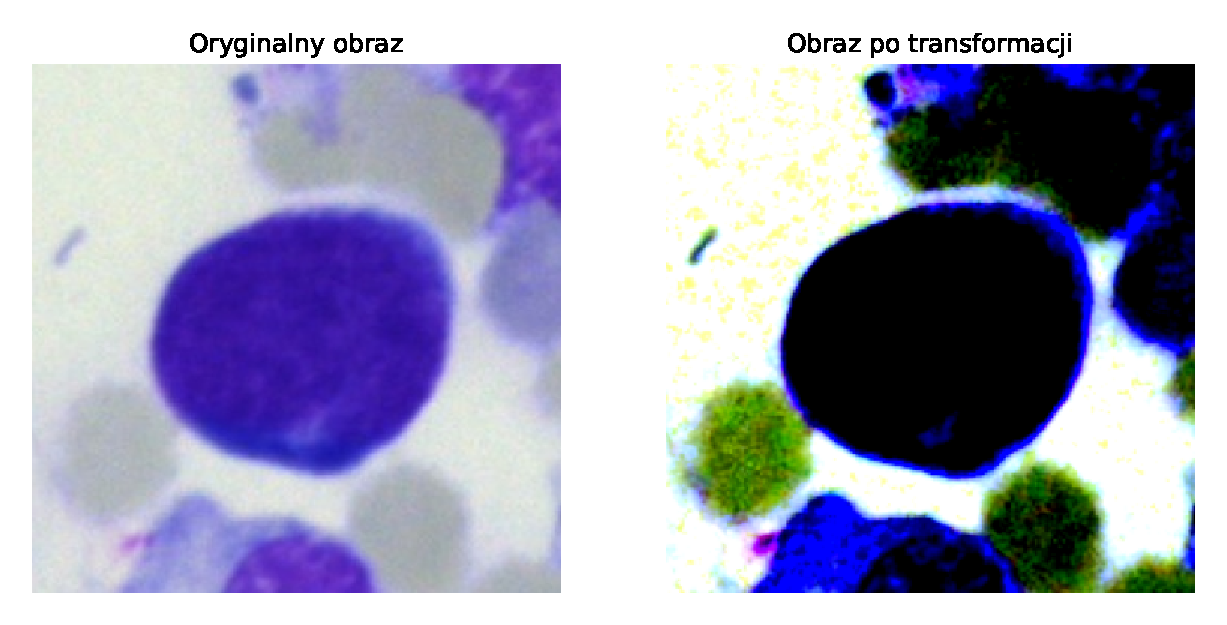
\includegraphics[width=\textwidth]{image_transform}
    \caption{Porównanie obrazu wejściowego przed i po transformacji}
    \label{fig:transformations_example}
\end{figure}

Po przetwarzaniu zbiór danych został podzielony losowo na zestaw treningowy i walidacyjny w proporcjach odpowiednio \textit{80:20}.
Zestaw treningowy służy do optymalizacji parametrów sieci neuronowej.
Zestaw walidacyjny natomiast jest używany do sprawdzania jakości modelu na obrazach, których sieć neuronowa "nigdy nie widziała".

\subsection{Trening sieci neuronowej}

Niniejsza praca ma za zadanie między innymi porównać różne architektury splotowych sieci neuronowych i ocenić,
która z nich wypada najlepiej w zadaniu klasyfikacji komórek z rozmazów szpiku kostnego.
Omówiony poniżej trening sieci neuronowej o architekturze \textit{EfficientNet B0} wygląda tak samo dla innych architektur, takich jak \textit{EfficientNet B5}, \textit{ResNet} i innych.
Współczynnik uczenia wynosił \textit{0.001}, a ilość epok była równa 3.
\textcolor{red}{Niestety z powodu ograniczeń infrastruktury do trenowania, nie udało się wykonać walidacji krzyżowej dla każdego z modeli osobno. Zbiór walidacyjny był natomiast wybierany losowo za każdym razem, gdy badano nową sieć neuronową.}

Trenowanie sieci neuronowej z użyciem biblioteki PyTorch sprowadza się do iterowania po zbiorze wejściowym i wykonywania kroku optymalizacyjnego przy każdym przejściu.
Uproszczony schemat działania głównej pętli treningowej (kod przestawiony na listingu~\ref{lst:train}):

\begin{enumerate}
    \item Pobranie miniwsadu z próbkami treningowymi i skopiowanie ich na urządzenie zewnętrzne, czyli kartę graficzną.
    \item Wykonanie przejścia w przód sieci neuronowej.
    Oznacza to obliczenie wartości neuron na warstwie wyjściowej na bazie uprzednio pobranych próbek.
    \item Porównanie wyjścia sieci neuronowej z oczekiwanymi predykcjami i obliczenie błędu sieci.
    \item Obliczenie gradientów za pomocą algorytmu propagacji wstecznej.
    \item Wykonanie kroku optymalizacyjnego z użyciem optymalizatora \textit{Adam}.
    \item Obliczenie metryk dla zbioru walidacyjnego i zapisanie ich.
\end{enumerate}

\lstinputlisting[label={lst:train}, caption={Kod pętli treningowej w języku Python z wykorzystaniem PyTorch}, language=ipython]{train.py}

\subsection{Ewaluacja jakości modelu}

\begin{figure}
    \centering
    \includegraphics[width=0.5\textwidth]{cam}
    \caption{Mapa cieplna GradCAM dla obrazu komórki plazmatycznej}
    \label{fig:cam}
\end{figure}


Wyjściem modelu jest rozkład prawdopodobieństwa rozpoznania poszczególnych rodzajów komórek oraz mapa cieplna GradCAM.
Przykładowa mapa cieplna jest widoczna na rys.~\ref{fig:cam}.
Przedstawia ona miejsca na obrazie, które najbardziej wpłynęły na predykcję.
\textcolor{green}{
    Zgadzają się one z obszarami, na które zwraca uwagę lekarz - sprawdza on wygląd jądra komórkowego jak i jego ziarnistości.
}

Do sprawdzenia jakości modelu uczenia maszynowego konieczny jest dobór właściwych metryk.
Ze względu na to, że trenowany jest klasyfikator wieloklasowy, a zbiór danych nie jest zrównoważony, zwykłe metryki takie jak dokładność (z ang. \textit{accuracy}) nie wystarczą.
Dla każdej klasy jest liczona precyzja (z ang. \textit{precision}) i czułość (z ang. \textit{recall}).
Obie te metryki składają się do obliczenia wyniku F1 (z ang. \textit{F1-score})~\cite{geron}.
Co ważne, wynik F1 jest liczony z uwzględnieniem wag poszczególnych klas.
Obliczana jest również macierz pomyłek.
Informuje ona o tym, które klasy są najczęściej mylone między sobą.
Metryki są zapisywane do pliku tekstowego oraz do plików obrazów w celu późniejszej analizy.


\section{Interfejs użytkownika}

W celu łatwego korzystania z modelu uczenia maszynowego przez diagnostów \textcolor{red}{opracowana została} aplikacja internetowa do interakcji z nim.
Zrzut ekranu interfejsu użytkownika jest widoczny na rys.~\ref{fig:ui}.
Aplikacja została napisana z użyciem \textit{Vue}~\cite{vue} - biblioteki do tworzenia interaktywnych interfejsów użytkownika dla sieci web.
Łączy się ona z serwerem HTTP napisanym z użyciem biblioteki Flask~\cite{flask}.
Serwer eksponuje interfejs REST API, który dla wysłanego zdjęcia zwraca rozkład prawdopodobieństwa \textcolor{red}{ rozpoznania poszczególnych klas}.
Przed wywołaniem modelu, funkcja upewnia się, że przychodzący obrazek jest poprawnego formatu.
Dopiero po zwalidowaniu poprawności danych, kod przystępuje do utworzenia rozkładu prawdopodobieństwa (zmienna \textit{result}).
Renderowana jest również mapa cieplna GradCAM informująca użytkownika o regionach obrazu, które były kluczowe dla modelu w trakcie wykonywania predykcji.


\begin{figure}
    \centering
    \includegraphics[width=\textwidth]{app}
    \caption{Aplikacja internetowa do rozpoznawania komórek}
    \label{fig:ui}
\end{figure}


\begin{figure}
    \centering
    \includegraphics[width=0.8\textwidth]{arch}
    \caption{Architektura klient-serwer aplikacji internetowej i serwera Flask}
    \label{fig:arch}
\end{figure}

By skorzystać z aplikacji internetowej, należy przeciągnąć plik ze zdjęciem komórki do sekcji "Upuść tutaj rozmaz w PNG lub JPEG".
Po wysłaniu obrazu użytkownik może wybrać model i kliknąć przycisk "Rozpoznaj rodzaj komórki".
Następnie ukaże się tabela z rozkładem prawdopodobieństwa (po prawej stronie okna).
Stylizowanie aplikacji zostało wykonane z użyciem biblioteki CSS o nazwie \textit{Tailwind.css}~\cite{tailwind}.
Komunikacja klient-serwer jest zapewniona przez bibliotekę \textit{Axios}~\cite{axios}.
Architekturę przedstawia rys.~\ref{fig:arch}.


\section{Algorytm ekstrakcji obrazów komórek z dużego zdjęcia rozmazu}\label{sec:kwadraty}

Zbiór danych użyty w trakcie trenowania splotowej sieci neuronowej przedstawia komórki, które zajmują prawie całą cześć obrazu.
Innymi słowy, każdy obrazek stanowi wycinek dużego skanu z rozmazu.
Często jednak istnieje potrzeba zautomatyzowania procesu wycinania kwadratowych obrazów przedstawiających komórki z dużego skanu.
Zaproponowano algorytm korzystający z różnych metod wizji komputerowej do osiągnięcia tego zadania.

Niniejszy algorytm przyjmuje obraz przedstawiający kilkanaście komórek różnego rodzaju i eksportuje
każdą komórkę do kwadratowego zdjęcia.
Algorytm wykonuje następujące kroki w celu wyznaczenia komórek z obrazka:

\begin{figure}
    \centering
    \includegraphics[width=0.8\textwidth]{Im060_1}
    \caption{Wejście algorytmu}
    \label{fig:extract_input}
\end{figure}

\begin{figure}
    \centering
    \includegraphics[width=0.8\textwidth]{Im060_1_thresh}
    \caption{Obrazek po progowaniu}
    \label{fig:extract_thresh}
\end{figure}

\begin{figure}
    \centering
    \includegraphics[width=0.8\textwidth]{Im060_1_contours}
    \caption{Oznaczone kontury wraz z punktami centralnymi}
    \label{fig:extract_contours}
\end{figure}

\begin{figure}
    \centering
    \includegraphics[width=0.8\textwidth]{cells}
    \caption{Wyekstraktowane kwadratowe obrazki}
    \label{fig:extract_squares}
\end{figure}

\begin{enumerate}
    \item Konwersja oryginalnego obrazu (rys.~\ref{fig:extract_input}) na skalę szarości.
    Jest to konieczne, ponieważ progowanie w kroku drugim nie może odbywać się na obrazie kolorowym.
    Do konwersji zastosowano funkcję \textit{cv2.cvtColor} - pozwala ona konwertować obraz z jednej przestrzeni kolorów do innej.
    \item Progowanie z pomocą algorytmu Otsu~\cite{otsu}.
    Jest to algorytm adaptacyjnego progowania, często stosowany do analizy obrazów medycznych.
    Progowanie ma na celu wyodrębnienie ciemniejszych obszarów obrazu - cytoplazmy i jądra komórek (rys.~\ref{fig:extract_thresh}). Otsu jest algorytmem progowania globalnego i opiera się na analizie histogramu.
    Dąży on do maksymalizacji wariancji międzyklasowej.
    \item Wyznaczenie konturów z pomocą funkcji \textit{cv2.findContours}~\cite{contours}.
    Kontur jest definiowany jako pewna ciągła krzywa, która łączy punkty o tej samej intensywności.
    W opisanym algorytmie kontury mają za zadanie informować o granicach komórki.
    Argumentem funkcji jest flaga \textit{cv2.RETR\_EXTERNAL}, która powoduje, że zwrócone zostają jedynie najbardziej zewnętrzne kontury - kontury wewnętrzne są ignorowane.
    \item Obliczanie punktów centralnych konturów za pomocą momentów Hu. Każdy wyznaczony punkt centralny jest traktowany jako środek komórki (rys.~\ref{fig:extract_contours}).
    Współrzędne punktów centralnych można wyznaczyć na podstawie momentów Hu, korzystając ze wzorów~\ref{eq:hu_x} i~\ref{eq:hu_y}.
    \begin{equation}
        \bar{x} = \dfrac{M_{10}}{M_{00}}\label{eq:hu_x}
    \end{equation}
    \begin{equation}
        \bar{y} = \dfrac{M_{01}}{M_{00}}\label{eq:hu_y}
    \end{equation}
    \item Wycięcie obszaru komórki za pomocą indeksów Python (rys.~\ref{fig:extract_squares}). Obraz każdej znalezionej komórki trafia do osobnego pliku w folderze wyjściowym.
    Do zapisu na dysk wykorzystano funkcję \textit{matplotlib.pyplot.imsave()}.
\end{enumerate}

Kod opisanego algorytmu przedstawia listing~\ref{lst:extract}.

\lstinputlisting[label={lst:extract}, caption={Kod wycinający obraz komórki z dużego skanu mikroskopowego}, language=ipython]{extract.py}
    \chapter{Analiza wyników}


\section{Ocena jakości różnych architektur sieci neuronowych}

%\begin{table}
%    \caption{Porównanie jakości predykcji różnych architektur splotowych sieci neuronowych}
%    \begin{center}
%        \begin{tabular}{|l|l|l|l|l|}
%            \hline
%            Architektura             & Liczba parametrów & F1             & Wykresy funkcji błędu i F1     & Macierz pomyłek                     \\
%            \hline
%            EfficientNet B0          & 5.3M             & 0.860          & rys. \ref{fig:plot_efficientnet_b0} & rys. \ref{fig:confusion_efficientnet_b0} \\
%            \hline
%            EfficientNet B1          & 7.8M             & 0.850          & rys. \ref{fig:plot_efficientnet_b1} & rys. \ref{fig:confusion_efficientnet_b1} \\
%            \hline
%            EfficientNet B2          & 9.2M             & 0.860          & rys. \ref{fig:plot_efficientnet_b2} & rys. \ref{fig:confusion_efficientnet_b2} \\
%            \hline
%            EfficientNet B3          & 12.0M            & 0.870          & rys. \ref{fig:plot_efficientnet_b3} & rys. \ref{fig:confusion_efficientnet_b3} \\
%            \hline
%            \textbf{EfficientNet B4} & \textbf{19.0M}   & \textbf{0.880} & rys. \ref{fig:plot_efficientnet_b4} & rys. \ref{fig:confusion_efficientnet_b4} \\
%            \hline
%            EfficientNet B5          & 30.0M            & 0.860          & rys. \ref{fig:plot_efficientnet_b5} & rys. \ref{fig:confusion_efficientnet_b5} \\
%            \hline
%            DenseNet121              & 8.0M             & 0.850          & rys. \ref{fig:plot_densenet121}     & rys. \ref{fig:confusion_densenet121}     \\
%            \hline
%            DenseNet169              & 14.1M            & 0.840          & rys. \ref{fig:plot_densenet169}     & rys. \ref{fig:confusion_densenet169}     \\
%            \hline
%            DenseNet201              & 20.0M            & 0.850          & rys. \ref{fig:plot_densenet201}     & rys. \ref{fig:confusion_densenet201}     \\
%            \hline
%            ResNet18                 & 11.7M            & 0.840          & rys. \ref{fig:plot_resnet18}        & rys. \ref{fig:confusion_resnet18}        \\
%            \hline
%        \end{tabular}
%    \end{center}
%    \label{tab:comparison}
%\end{table}
\begin{table}
    \caption{Podsumowanie miary F1 dla poszczególnych klas (EfficientNet B4)}
    \begin{center}
        \begin{tabular}{|l|l|l|l|l|}
            \hline
            Klasa & Precyzja & Czułość & F1    & Liczba próbek \\
            \hline
            BLA   & 0.780    & 0.840   & 0.810 & 2311          \\
            \hline
            EBO   & 0.940    & 0.960   & 0.950 & 5532          \\
            \hline
            EOS   & 0.980    & 0.980   & 0.980 & 1192          \\
            \hline
            LYT   & 0.910    & 0.930   & 0.920 & 5193          \\
            \hline
            MON   & 0.720    & 0.730   & 0.720 & 825           \\
            \hline
            MYB   & 0.780    & 0.660   & 0.710 & 1323          \\
            \hline
            NGB   & 0.780    & 0.790   & 0.790 & 1962          \\
            \hline
            NGS   & 0.930    & 0.930   & 0.930 & 5984          \\
            \hline
            PEB   & 0.780    & 0.650   & 0.710 & 552           \\
            \hline
            PLM   & 0.940    & 0.860   & 0.900 & 1466          \\
            \hline
            PMO   & 0.830    & 0.840   & 0.840 & 2429          \\
            \hline
        \end{tabular}
    \end{center}
    \label{tab:f1_summary}
\end{table}

Niniejszy projekt ma za zadanie porównać różne architektury splotowych sieci neuronowych i wskazać, która z nich daje najlepsze rezultaty.
Dla każdej architektury wskazano jej wielkość (ilość parametrów trenowalnych) oraz ważony wynik F1.
Większy wynik F1 informuje o lepszym zachowaniu modelu w rozpoznawaniu typów komórek.

Warto zauważyć, że \textcolor{red}{często wielkość sieci neuronowej (liczba wag)} \textcolor{red}{nie jest liniowo zależna} z jakością uzyskiwanych predykcji.
Dzieje się tak ze względu na to, że pojemność zachowania informacji nawet w mniejszej sieci jest wystarczająca, by móc rozpoznawać rodzaje komórek.

\begin{figure}
    \centering
    \includegraphics[width=\textwidth]{experiments/efficientnet_b0/combined}
    \caption{Wykres zależności funkcji straty i F1 od epoki trenowania (EfficientNet B0)}
    \label{fig:plot_efficientnet_b0}
\end{figure}
\begin{figure}
    \centering
    \includegraphics[width=0.8\textwidth]{experiments/efficientnet_b0/confusion_matrix}
    \caption{Macierz pomyłek modelu EfficientNet B0}
    \label{fig:confusion_efficientnet_b0}
\end{figure}

\begin{figure}
    \centering
    \includegraphics[width=\textwidth]{experiments/efficientnet_b1/combined}
    \caption{Wykres zależności funkcji straty i F1 od epoki trenowania (EfficientNet B1)}
    \label{fig:plot_efficientnet_b1}
\end{figure}
\begin{figure}
    \centering
    \includegraphics[width=0.8\textwidth]{experiments/efficientnet_b1/confusion_matrix}
    \caption{Macierz pomyłek modelu EfficientNet B1}
    \label{fig:confusion_efficientnet_b1}
\end{figure}

\begin{figure}
    \centering
    \includegraphics[width=\textwidth]{experiments/efficientnet_b2/combined}
    \caption{Wykres zależności funkcji straty i F1 od epoki trenowania (EfficientNet B2)}
    \label{fig:plot_efficientnet_b2}
\end{figure}
\begin{figure}
    \centering
    \includegraphics[width=0.8\textwidth]{experiments/efficientnet_b2/confusion_matrix}
    \caption{Macierz pomyłek modelu EfficientNet B2}
    \label{fig:confusion_efficientnet_b2}
\end{figure}

\begin{figure}
    \centering
    \includegraphics[width=\textwidth]{experiments/efficientnet_b3/combined}
    \caption{Wykres zależności funkcji straty i F1 od epoki trenowania (EfficientNet B3)}
    \label{fig:plot_efficientnet_b3}
\end{figure}
\begin{figure}
    \centering
    \includegraphics[width=0.8\textwidth]{experiments/efficientnet_b3/confusion_matrix}
    \caption{Macierz pomyłek modelu EfficientNet B3}
    \label{fig:confusion_efficientnet_b3}
\end{figure}

\begin{figure}
    \centering
    \includegraphics[width=\textwidth]{experiments/efficientnet_b4/combined}
    \caption{Wykres zależności funkcji straty i F1 od epoki trenowania (EfficientNet B4)}
    \label{fig:plot_efficientnet_b4}
\end{figure}
\begin{figure}
    \centering
    \includegraphics[width=0.8\textwidth]{experiments/efficientnet_b4/confusion_matrix}
    \caption{Macierz pomyłek modelu EfficientNet B4}
    \label{fig:confusion_efficientnet_b4}
\end{figure}

\begin{figure}
    \centering
    \includegraphics[width=\textwidth]{experiments/efficientnet_b5/combined}
    \caption{Wykres zależności funkcji straty i F1 od epoki trenowania (EfficientNet B5)}
    \label{fig:plot_efficientnet_b5}
\end{figure}
\begin{figure}
    \centering
    \includegraphics[width=0.8\textwidth]{experiments/efficientnet_b5/confusion_matrix}
    \caption{Macierz pomyłek modelu EfficientNet B5}
    \label{fig:confusion_efficientnet_b5}
\end{figure}

\begin{figure}
    \centering
    \includegraphics[width=\textwidth]{experiments/densenet121/combined}
    \caption{Wykres zależności funkcji straty i F1 od epoki trenowania (DenseNet121)}
    \label{fig:plot_densenet121}
\end{figure}
\begin{figure}
    \centering
    \includegraphics[width=0.8\textwidth]{experiments/densenet121/confusion_matrix}
    \caption{Macierz pomyłek modelu DenseNet121}
    \label{fig:confusion_densenet121}
\end{figure}

\begin{figure}
    \centering
    \includegraphics[width=\textwidth]{experiments/densenet169/combined}
    \caption{Wykres zależności funkcji straty i F1 od epoki trenowania (DenseNet169)}
    \label{fig:plot_densenet169}
\end{figure}
\begin{figure}
    \centering
    \includegraphics[width=0.8\textwidth]{experiments/densenet169/confusion_matrix}
    \caption{Macierz pomyłek modelu DenseNet169}
    \label{fig:confusion_densenet169}
\end{figure}

\begin{figure}
    \centering
    \includegraphics[width=\textwidth]{experiments/densenet201/combined}
    \caption{Wykres zależności funkcji straty i F1 od epoki trenowania (DenseNet201)}
    \label{fig:plot_densenet201}
\end{figure}
\begin{figure}
    \centering
    \includegraphics[width=0.8\textwidth]{experiments/densenet201/confusion_matrix}
    \caption{Macierz pomyłek modelu DenseNet201}
    \label{fig:confusion_densenet201}
\end{figure}

\begin{figure}
    \centering
    \includegraphics[width=\textwidth]{experiments/resnet18/combined}
    \caption{Wykres zależności funkcji straty i F1 od epoki trenowania (ResNet18)}
    \label{fig:plot_resnet18}
\end{figure}
\begin{figure}
    \centering
    \includegraphics[width=0.8\textwidth]{experiments/resnet18/confusion_matrix}
    \caption{Macierz pomyłek modelu ResNet18}
    \label{fig:confusion_resnet18}
\end{figure}

\subsection{EfficientNet B0}
\textit{Liczba parametrów: 5.3M}

\textit{Ważony wynik F1: 0.860}

Najmniejszy wariant architektury EfficientNet, zawierający tylko 5.3M parametrów oferuje jakość predykcji na poziomie ważonego wyniku F1 równego 0.86.
Na podstawie wykresu 4.1 można stwierdzić, że już pierwsza epoka treningu sieci daje satysfakcjonujące rezultaty (wyk.~\ref{fig:plot_efficientnet_b0}).
Kolejne dwie epoki jedynie nieznacznie poprawiają jakość modelu.
Najczęściej mylonymi klasami jest klasa NGB (Krwinka biała pałeczkowata) i NGS (Segmentowany neutrofil) - rys.~\ref{fig:confusion_efficientnet_b0}.

\subsection{EfficientNet B1}
\textit{Liczba parametrów: 7.8M}

\textit{Ważony wynik F1: 0.850}

Dla treningu wariantu B1 architektury EfficientNet zachodzi lekkie przetrenowanie.
Na podstawie wykresu F1 (wyk.~\ref{fig:plot_efficientnet_b1}) można zobaczyć, że trenowanie w trzeciej epoce jedynie pogarsza jakość predykcji.
Sieć często myli klasy PEB (Proerytroblast) z EBO (Erytroblast) i NGB (Krwinka biała pałeczkowata) z NGS (Segmentowany neutrofil) - rys. ~\ref{fig:confusion_efficientnet_b1}.

\subsection{EfficientNet B2}
\textit{Liczba parametrów: 9.2M}

\textit{Ważony wynik F1: 0.860}

Architektura EfficientNet B2 dostarcza dostatecznej jakości prognoz już w pierwszej epoce treningu.
Kolejne epoki jedynie nieznacznie poprawiają jakość modelu (wyk.~\ref{fig:plot_efficientnet_b2}).
Najczęściej mylonymi klasami są MYB (Mielocyt) i PMO (Promielocyt) - rys.~\ref{fig:confusion_efficientnet_b2}.

\subsection{EfficientNet B3}
\textit{Liczba parametrów: 12.0M}

\textit{Ważony wynik F1: 0.870}

Proces treningu EfficientNet B3 wygląda bardzo podobnie jak trening EfficientNet B2. Model natomiast charakteryzuje się nieco lepszą miarą F1 równą 0.87 w porównaniu do 0.86 modelu B2 (wyk.~\ref{fig:plot_efficientnet_b3}). Najczęściej mylonymi klasami są MYB (Mielocyt) i PMO (Promielocyt), oraz EBO (Erytroblast) i PEB (Proerytroblast) - rys.~\ref{fig:confusion_efficientnet_b3}.

\subsection{EfficientNet B4}
\textit{Liczba parametrów: 19.0M}

\textit{Ważony wynik F1: 0.880}

Jest to najlepszy model uzyskany w trakcie badań projektu inżynierskiego.
Jego wynik F1 wynosi 0.88 (wyk.~\ref{fig:plot_efficientnet_b4}). Najczęściej mylonymi klasami są MYB (Mielocyt) i PMO (Promielocyt) - rys.~\ref{fig:confusion_efficientnet_b4}.
Tabela ~\ref{tab:f1_summary} przedstawia zestawienie precyzji, czułości i F1 dla poszczególnych klas.

\subsection{EfficientNet B5}
\textit{Liczba parametrów: 30.0M}

\textit{Ważony wynik F1: 0.860}

Pomimo tego, że model ten zawiera więcej parametrów niż EfficientNet B4, miara F1 wynosi 0.86, co oznacza, że jego predykcje są gorsze niż w przypadku EfficientNet B4 (wyk.~\ref{fig:plot_efficientnet_b5}).
Najczęściej mylonymi klasami są MYB (Mielocyt) i PMO (Promielocyt) - rys.~\ref{fig:confusion_efficientnet_b5}.

\subsection{DenseNet121}
\textit{Liczba parametrów: 8.0M}

\textit{Ważony wynik F1: 0.850}

Architektura DenseNet121 trenuje się podobnie jak architektury EfficientNet - to znaczy już w pierwszej epoce treningu ważony wynik F1 jest bliski temu po trzeciej epoce (wyk.~\ref{fig:plot_densenet121}).
Najczęściej mylonymi klasami są NGB (Krwinka biała pałeczkowata) i NGS (Segmentowany neutrofil) oraz MYB (Mielocyt) i PMO (rys.~\ref{fig:confusion_densenet121}).

\subsection{DenseNet169}
\textit{Liczba parametrów: 14.1M}

\textit{Ważony wynik F1: 0.840}

Sieć głównie trenuje się w pierwszej epoce, dwie kolejne nieznacznie poprawiają jej jakość.
W trzeciej epoce widać oznaki nadmiernego dopasowania (wyk.~\ref{fig:plot_densenet169}).
Najczęściej mylonymi klasami są MON (Monocyt) i BLA (Blast) oraz MYB (Mielocyt) i PMO (Promielocyt) - rys.~\ref{fig:confusion_densenet169}.

\subsection{DenseNet201}
\textit{Liczba parametrów: 20.0M}

\textit{Ważony wynik F1: 0.850}

Przebieg treningu DenseNet201 przypomina trening DenseNet169.
Po trzeciej epoce nie występuje jednak nadmierne dopasowanie (wyk.~\ref{fig:plot_densenet201}), a najczęściej mylonymi klasami są MON (Monocyt) i BLA (Blast) oraz MYB (Mielocyt) i PMO (Promielocyt) - rys.~\ref{fig:confusion_densenet201}.

\subsection{ResNet18}
\textit{Liczba parametrów: 11.7M}

\textit{Ważony wynik F1: 0.840}

Architektura ResNet18, zawierając 11.7M parametrów oferuje gorszą jakość predykcji (wyk.~\ref{fig:plot_resnet18}) niż przykładowo EfficientNet B2, która posiada 9.2M parametrów (ważony wynik F1 sieci ResNet wynosi 0.84 w porównaniu do 0.86 sieci EfficientNet B2).
Najczęściej mylonymi klasami są MYB (Mielocyt) i PMO (Promielocyt) - rys.~\ref{fig:confusion_resnet18}.

\newline
\newline
\newline

%TODO net
Najlepsze wyniki uzyskuje model używający architektury \textit{EfficientNet B4}.
Ważony wynik F1 w jej przypadku wynosi \textit{0.88}.

\textcolor{red}{
    Na podstawie wykresów funkcji straty i F1, można stwierdzić, że dla wszystkich sieci neuronowych już pierwsza epoka skutkowała rozpoznaniem wzorców.
    Kolejne epoki nie poprawiały \textcolor{green}{znacząco} skuteczności sieci.
    Często mylonymi komórkami były promielocyty (\textit{PMO}) i mielocyty (\textit{MYB}), wynika to z tego, że ich wygląd jest podobny.
}


\section{Porównanie z innymi algorytmami}

\begin{figure}
    \centering
    \includegraphics[width=0.6\textwidth]{resnext_confusion_matrix}
    \caption{Macierz pomyłek dla modelu ResNeXt \cite{resnext}}
    \label{fig:resnext_confusion_matrix}
\end{figure}

Dostawca zbioru danych, w artykule \textit{Highly accurate differentiation of bone marrow cell morphologies using deep neural networks on a large image dataset} \cite{resnext} wykorzystuje architekturę \textit{ResNetXt-50}.
Model zawierający ponad 23 miliony parametrów był trenowany na \textit{NVIDIA TESLA V100} przez ok. 48 godzin.
Podobnie jak w niniejszym projekcie, autorzy artykułu wykonali normalizację intensywności kolorów przed trenowaniem sieci neuronowej (z powodu różnic w barwieniu Maya-Grünwalda-Giemsa).
Uzyskany ważony wynik F1 dla architektury \textit{ResNeXt-50} wyniósł \textit{0.822}.
Macierz pomyłek dostarczona przed autorów pracy jest widoczna na rys. \ref{fig:resnext_confusion_matrix}.


\section{Wyzwania}

Głównym wyzwaniem w trakcie realizacji projektu było wytrenowanie dużych sieci neuronowych.
Niestety, ich trening na lokalnym sprzęcie takim jak komputer osobisty jest bardzo czasochłonny.
W związku z tym konieczne było uruchamianie ich na platformie \textit{kaggle.com}, która oferuje 30 godzin czasu procesora graficznego miesięcznie.
Nieodpłatna możliwość pracy na platformie pozwoliła na pomyślną realizację projektu.


\section{Wnioski}

%TODO net
Zaprezentowane porównanie różnych splotowych sieci neuronowych pokazuje, że najlepszym modelem do zadania klasyfikacji rodzajów komórek w szpiku kostnym jest \textit{EfficientNet B4}.
Wybrana sieć neuronowa uzyskuje najlepszy ważony wynik F1 równy \textit{0.88}.
Warto też zwrócić uwagę na to, że sieci neuronowe znacznie większe od \textit{EfficientNet B4} nie dawały dużo lepszych rezultatów.


    \chapter{Podsumowanie}

W niniejszym projekcie inżynierskim omówiono realizację systemu klasyfikatora rodzajów komórek szpiku kostnego na podstawie uczenia maszynowego.
Porównane zostały różne architektury splotowych sieci neuronowych.
Architekturą, która daje najlepsze rezultaty okazała się \textbf{EfficientNet B4}.
Przedstawione rozwiązanie oferuje podobną jakość klasyfikacji (uwzględniając ważoną miarę F1) co inne, uprzednio opublikowane prace naukowe.
Warto zauważyć jednak, że sieć EfficientNet B4 dostarcza podobnej jakości predykcji co omawiana w innych artykułach architektura \textit{ResNeXt}, mimo że ilość parametrów do wyuczenia jest znacznie mniejsza (19 milionów parametrów w przypadku EfficientNet B4 versus 25 milionów w przypadku ResNeXt \cite{resnext}).

Opisano również algorytm ekstrakcji obrazów komórek z dużego skanu rozmazu, dzięki któremu można automatycznie wyznaczyć dane wejściowe do sieci neuronowej (sieć neuronowa wymaga obrazu pojedynczej komórki).
Do jego opracowania wykorzystano takie metody widzenia komputerowego jak progowanie, znajdowanie konturów czy momenty Hu.

W ramach projektu stworzono również przejrzysty interfejs użytkownika, który umożliwia użytkownikowi łatwą interakcję z modelem sztucznej inteligencji.
Po wysłaniu obrazu komórki na serwer pojawia się tabela rozkładu prawdopodobieństwa wraz z wizualizacją mapy cieplnej \textit{GradCam}.
Mapa cieplna pozwala użytkownikowi lepiej zrozumieć proces predykcji klas.

Podsumowując, zaprezentowany system stanowi przykład praktycznego zastosowania uczenia maszynowego i splotowych sieci neuronowych w medycynie.
W świetle obecnego tempa rozwoju technik sztucznej inteligencji, można się spodziewać, że w przyszłości rozwiązania oparte o SI będą rozwiązywały coraz to bardziej złożone problemy w wielu branżach i dziedzinach życia.
Wynikająca z tego automatyzacja będzie prowadziła do przyspieszenia różnych procesów oraz oszczędności wielu godzin pracy specjalistów.

    % itd.
    % \appendix
    % \include{dodatekA}
    % \include{dodatekB}
    % itd.

    \printbibliography

\end{document}
